% RECON-OMEGA: Doctoral Research Proposal (research plan; no model experiments claimed).
% Maintains the user's RECON Overleaf visual grammar and typography.
% Compile: pdflatex main.tex twice (or latexmk -pdf main.tex).
\documentclass[11pt,a4paper]{article}
\usepackage[utf8]{inputenc}
\usepackage[T1]{fontenc}
\usepackage{lmodern}
\usepackage[a4paper,left=24mm,right=24mm,top=23mm,bottom=23mm,headheight=14pt,headsep=6mm,footskip=12mm]{geometry}
\usepackage{amsmath,amssymb,amsthm,mathtools,bm,booktabs,tabularx,array,graphicx,enumitem,multirow,makecell}
\usepackage{tikz}
\usetikzlibrary{arrows.meta,calc,positioning,fit,backgrounds}
\usepackage{fancyhdr,algorithm,algpseudocode,xcolor,caption,subcaption,needspace}
\usepackage[numbers,sort&compress]{natbib}
\usepackage[hypertexnames=false,colorlinks=true,linkcolor=blue!50!black,urlcolor=blue!55!black,citecolor=blue!50!black]{hyperref}
\usepackage[nameinlink,noabbrev]{cleveref}
\hypersetup{pdftitle={RECON-Omega: Certifiable Causal Recovery of Scientific Competence Hypergraphs},pdfauthor={Mohammad Amanlou},pdfsubject={Doctoral research proposal, November 2026}}
\urlstyle{same}
\pagestyle{fancy}\fancyhf{}
\fancyhead[L]{\small\itshape RECON-$\Omega$: Causal competence discovery}
\fancyhead[R]{\small Mohammad Amanlou}
\fancyfoot[C]{\small\thepage}
\renewcommand{\headrulewidth}{0.3pt}
\setlength{\parindent}{0pt}\setlength{\parskip}{5pt plus .7pt minus .5pt}
\setlength{\emergencystretch}{2em}
\setlist[itemize]{leftmargin=1.35em,topsep=3pt,itemsep=2pt,parsep=0pt}
\setlist[enumerate]{leftmargin=1.6em,topsep=2pt,itemsep=2pt,parsep=0pt}
\setlength{\abovedisplayskip}{8pt plus 2pt}\setlength{\belowdisplayskip}{8pt plus 2pt}
\raggedbottom
\newcolumntype{Y}{>{\raggedright\arraybackslash}X}
\definecolor{aqua}{HTML}{146E70}\definecolor{rust}{HTML}{9C4E25}
\definecolor{iris}{HTML}{594B87}\definecolor{inkfig}{HTML}{233441}
\definecolor{lightbg}{HTML}{F3F7F9}
\newcommand{\E}{\mathbb{E}}\newcommand{\Prb}{\mathbb{P}}
\newcommand{\R}{\mathbb{R}}\newcommand{\N}{\mathbb{N}}
\newcommand{\A}{\mathcal{A}}\newcommand{\M}{\mathcal{M}}
\newcommand{\Hh}{\mathcal{H}}\newcommand{\V}{\mathcal{V}}
\newcommand{\F}{\mathcal{F}}\newcommand{\D}{\mathcal{D}}
\newcommand{\KL}{\mathrm{KL}}\newcommand{\TV}{\mathrm{TV}}
\newcommand{\ind}{\mathbf{1}}\newcommand{\supp}{\mathrm{supp}}
\newcommand{\proj}{\mathrm{Proj}}\newcommand{\argmin}{\operatorname*{arg\,min}}
\newcommand{\argmax}{\operatorname*{arg\,max}}
\newcommand{\txt}[1]{\textit{#1}}
\newtheorem{theorem}{Theorem}[section]
\newtheorem{proposition}[theorem]{Proposition}
\newtheorem{corollary}[theorem]{Corollary}
\newtheorem{lemma}[theorem]{Lemma}
\theoremstyle{definition}\newtheorem{definition}[theorem]{Definition}
\theoremstyle{remark}\newtheorem{remark}[theorem]{Remark}
\algrenewcommand\algorithmicrequire{\textbf{Input:}}
\algrenewcommand\algorithmicensure{\textbf{Output:}}
\begin{document}
\thispagestyle{plain}
{\sffamily\small DOCTORAL RESEARCH PROPOSAL\hfill NOVEMBER 2026\par}
\vspace{3mm}\hrule height .6pt\vspace{5mm}
{\fontsize{23}{27}\selectfont\bfseries RECON-$\Omega$: Scientific Skill\\ Dependencies and Their Identifiability\par}
\vspace{3mm}
{\large \textcolor{aqua}{Certifiable Causal Recovery of Higher-Order Competence Hypergraphs}\\[2pt]
\normalsize Controlled acquisition, functional lesions, selective relearning, and active experiments\par}
\vspace{5mm}{\large\textbf{Mohammad Amanlou}\par}
{\normalsize Prepared for scientific discussion with Prof. Andrey Ustyuzhanin, Constructor Knowledge Labs\par}
{\small \textit{Research proposal---theoretical results are conditional; open-weight experiments are planned, not reported.}\par}
\vspace{3mm}
\begin{center}\begin{minipage}{.95\linewidth}\small
\textbf{Abstract.} We propose to recover \emph{which combinations of scientific skills causally support transferable competence}, not merely which descriptions co-occur in documents or which questions a model answers. RECON-$\Omega$ compiles scientific sources into executable test worlds and performs randomized \emph{acquisition}, \emph{functional lesion}, and \emph{selective relearning} interventions on independent learner copies. The scientific target is a state- and protocol-indexed \emph{competence hypergraph}: its edges represent higher-order interventional effects, while a separate antichain records all minimal evidence packets sufficient for a prespecified gain on unseen compositions. We distinguish protocol-level causal effects from claims about unobserved internal mechanisms. Under an explicitly calibrated cross-channel response model, we establish (i) a noiseless multiskill identification result and a constructive failure of any fixed two-channel menu, (ii) a robust sparse-support recovery guarantee under projected separation and bounded intervention error, and (iii) an anytime-valid certificate under adaptive data collection. We prove precise limitations as well: uncalibrated lesions, insufficient experiment support, or indistinguishable mechanisms preclude structural identification regardless of sample size. A cost-aware experiment designer chooses tests to shrink the remaining ambiguity; an overidentifying fourth intervention is held out to \emph{falsify}, not merely fit, the assumed channel structure. The decisive evaluation uses programmable learners, independently checkable scientific programs, small trained transformers, and eventually open-weight LMs. Relative to existing factorial design, latent-capability learning, and unlearning work, the proposed contribution is a calibrated, interventionally testable \emph{identification target and certification procedure}, contingent on successful prospective neural validation. Human evaluation is optional.
\end{minipage}\end{center}
\vspace{2mm}
\begin{figure}[htbp]\centering
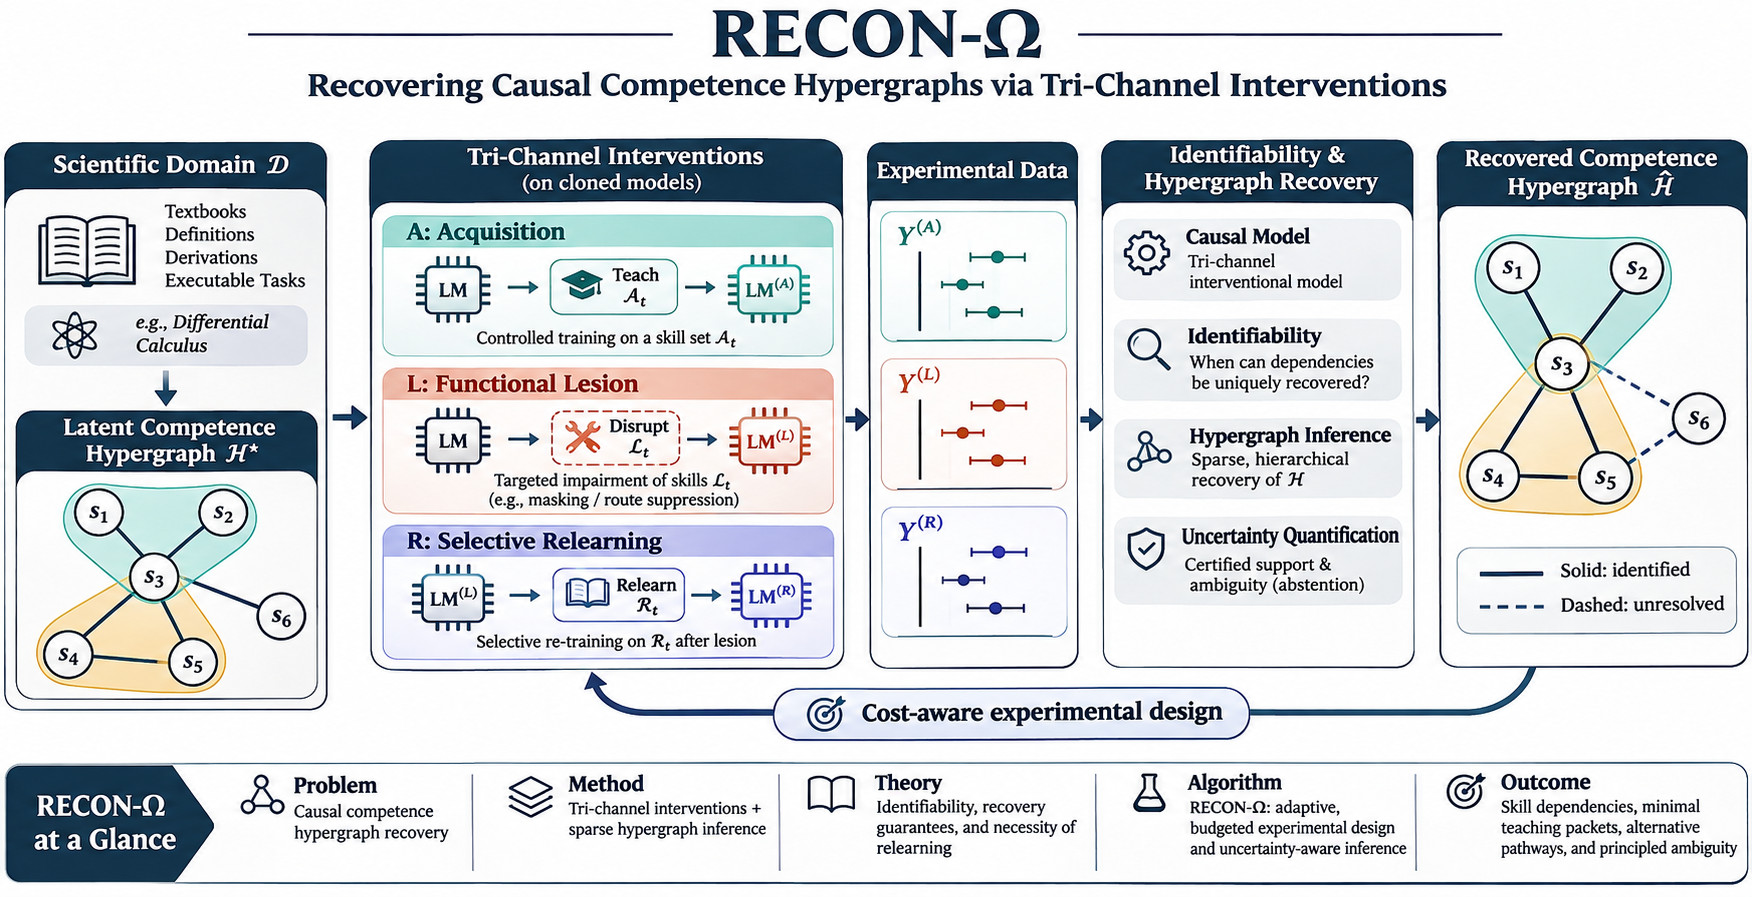
\includegraphics[width=\textwidth]{figures/recon_omega_overview.jpg}
\caption{\textbf{RECON-$\Omega$ at a glance.} Original research illustration generated for this proposal. Candidate skill dependencies are compiled from scientific sources and interrogated under three randomized intervention families. A fourth blinded perturbation tests the fitted cross-channel assumptions. Solid discovered dependencies would require statistical support; schematic edges in this figure do \emph{not} represent empirical findings.}\label{fig:overview}
\end{figure}

\clearpage
\thispagestyle{fancy}
{\sffamily\small\textcolor{aqua}{ONE-PAGE RESEARCH SUMMARY}\hfill RECON-$\Omega$\\[4pt]}
{\fontsize{18}{22}\selectfont\bfseries Research vision and methodological roadmap\par}
\vspace{2mm}\hrule height .6pt\vspace{3mm}
\begingroup\small\setlength{\parskip}{3pt}
\textbf{Scientific challenge.} Similar scores on scientific tasks can conceal incompatible mechanisms: genuine composition of mathematical skills, shortcut memorization, alternative reasoning paths, or residual knowledge hidden by an ineffective lesion. Neither textual prerequisites nor observational benchmark correlations establish which scientific explanations \emph{cause} reliable transfer. RECON-$\Omega$ asks which \emph{sets} of skills and which \emph{ordered intervention histories} causally change a specified learner's unaided performance on novel scientific compositions---and when the available experiments cannot distinguish rival explanations.

\textbf{What the project produces.} A source-grounded, state-indexed \emph{functional competence hypergraph} with calibrated effect intervals, alternative minimal sufficient teaching packets, and explicit unresolved dependencies. A stronger mechanistic interpretation is allowed only under independently tested intervention-calibration assumptions. Target tasks are executable scientific programs and novel symbolic-rule compositions; human studies are optional, not prerequisites for the primary contribution.

\vspace{2mm}
\begin{center}\renewcommand{\arraystretch}{1.17}\small
\begin{tabularx}{\linewidth}{>{\bfseries\color{aqua}}p{.18\linewidth}Y}
\toprule
Source compiler & Link textbook rules to typed skill candidates, controlled evidence packets, provenance, exact executable verifiers, and structurally disjoint transfer tests. \\
Experimental triad & Randomize \textbf{acquisition} (teach or filler), \textbf{functional lesion} (targeted mask or sham), and \textbf{selective relearning} after fixed disruption on independent model copies; audit collateral effects and preserved knowledge. \\
Causal estimands & Measure protocol-specific contrasts; recover higher-order interactions with bounded-arity M\"obius coefficients. Distinguish these effects from a potentially nonunique family of minimal gain-sufficient packets. \\
Identification & Use calibrated cross-channel restrictions, sparse recovery under explicit separation and bias bounds, and a fourth blinded perturbation that can \emph{falsify} the structural assumptions. Report partial identification when support is insufficient. \\
Experiment policy & Choose interventions under measured compute cost using a predictive surrogate, robust disagreement, and anytime-valid confidence sets; compare fairly against optimized factorial and cost-aware designs. \\
Evaluation & Benchmark with planted programmable worlds, independently verified scientific tasks, trainable modular and transformer learners, and later matched open-weight checkpoints; hold out worlds, motifs, seeds, and intervention protocols. \\
\bottomrule
\end{tabularx}
\end{center}
\vspace{1mm}
\textbf{Core technical question.} Let $\Omega_S^{(j)}(z)$ be the randomized higher-order contrast for skill set $S$ under experimental channel $j\in\{A,L,R\}$ at pre-intervention state $z$. Can a calibrated family $m_S=B w_S+e_S$ identify a shared functional dependency $\theta_S=c^\top w_S$ in the presence of alternative routes and off-target damage? The project supplies \emph{conditional} row-space/robust-support identification results, an adaptive selection procedure, and uncertainty certificates; broader sample-efficient recovery under unknown neural calibration remains a research target.

\textbf{Decision criterion and boundaries.} Success requires prospective intervention prediction and equal-cost improvements over strong factorial/pure-exploration competitors, with independent confirmation and correct uncertainty. Synthetic consistency is \emph{not} evidence of neural causal identification; reversible masking is \emph{not} verified unlearning. A failed calibration or matched-baseline tie narrows the claim rather than being hidden.

\vspace{1mm}\textit{\small Relation to KNIGHT and CKL: KNIGHT supplies source-grounded question construction; RECON-$\Omega$ contributes an experimental, theory-centered competence-discovery layer aligned with scientific knowledge structures and autonomous experimentation.}
\endgroup
\clearpage
\tableofcontents
\clearpage
\section{Scientific motivation and the consequential gap}\label{sec:intro}
\subsection{The scientific question}
Two language models can correctly differentiate a composite program for entirely different reasons: one may propagate local derivatives and accumulate paths; another may match templates memorized during pretraining; a third may use a different yet valid computational route. Similar benchmark accuracy does not distinguish their competence mechanisms. The same issue arises when an autonomous agent reads a textbook and hypothesizes that $S=\{\text{chain rule},\text{graph traversal}\}$ is a prerequisite for reverse-mode differentiation. A source graph gives an \emph{epistemic hypothesis}, not experimental evidence that training these two skills is necessary, synergistic, or sufficient for a particular model at a particular state.

\textbf{Central question.} \emph{Can we recover, with specified confidence and calibrated interventions, the minimal and potentially alternative combinations of source-linked scientific skills that change a model's closed-book ability to generalize to unseen compositions---and know when competing competence mechanisms remain indistinguishable?}

Our research treats programmable learners and model checkpoints as experimental subjects, not students. A downstream science-learning agent is a \emph{consumer} of the inferred structure. The main contribution lies in causal machine learning, active scientific experimentation, and reliability of generative models. The scientific content connects to source-grounded knowledge structures and competence hypergraphs in Constructor Knowledge Labs' research agenda \citep{constructor}. The proposed system extends the source-to-question infrastructure of KNIGHT \citep{knight}, but KNIGHT is not assumed to have implemented causal skill identification.

\subsection{Three independent objects must not be conflated}
\textbf{(i) Scientific dependency graph.} The logical statement that a theorem invokes a lemma, or that an algorithm calls a primitive, may be proved from a source or executable specification. This is \emph{not} a causal claim about a learner.

\textbf{(ii) Functional teaching effects.} A packet $T$ causes a change in held-out performance relative to a matched counterfactual protocol. These effects depend on checkpoint, optimizer, exposure format, order, task distribution, and resources. This object is identifiable through randomization in a well-defined experimental population.

\textbf{(iii) Internal competence mechanisms.} A causal route or representation within a neural model is a structural explanation that requires extra assumptions and interventions. Equivalent intervention laws can hide incompatible internal accounts \citep{geiger,jaber,hu2025}. RECON-$\Omega$ reports a supported \emph{functional} hypergraph by default and a \emph{mechanistic} certificate only when calibrations and overidentifying tests permit.

\subsection{Falsifiable hypotheses rather than outcome promises}
\begin{enumerate}
\item \textbf{H1:} jointly observing acquisition, disruption, and recovery distinguishes some higher-order shared skill contributions that the best fixed two-family menu cannot, \emph{under calibrated loadings and equal budgets}.
\item \textbf{H2:} a sparse history-conditioned model improves \emph{prospective prediction} of untouched intervention outcomes beyond optimized factorial, skill-transfer, and pairwise baselines.
\item \textbf{H3:} a certificate-driven experimental policy reaches the same correct decision yield at lower total verified compute than channel-aware adaptive factorial and cost-sensitive pure-exploration baselines.
\item \textbf{H4:} the recovered knowledge-graph annotations improve choice of minimal explanations on new scientific tasks relative to source order, training-skill baselines, and random packets.
\end{enumerate}
None of H1--H4 is asserted to have been demonstrated on neural models. The primary research contribution \emph{fails} if the calibrated mechanism does not predict independent interventions, if the same method exists in a matched factorial baseline, or if neural lesion bias overwhelms the identification margin.

\section{Related work: what is already solved, and what remains}\label{sec:rw}
The most important intellectual constraint is that \emph{prerequisite discovery, combinatorial effects, machine teaching, model editing, and active experiment design are all substantial existing fields}. The claim is not that their ingredients are new; it is that this sharply defined, checkably calibrated \emph{joint identification target} may admit informative results and transferable algorithms not covered under equivalent assumptions.

\subsection{A strong prior-art matrix}
\begin{table}[htbp]\centering\footnotesize
\caption{Nearest work and the decisive test separating RECON-$\Omega$ from incremental recombination. ``New test'' refers to a \emph{proposed} experiment, not established superiority.}\label{tab:prior}
\begin{tabularx}{\linewidth}{@{}p{.21\linewidth}Y Y@{}}\toprule
\textbf{Area / nearest work}&\textbf{Already established}&\textbf{What RECON-$\Omega$ must additionally establish}\\\midrule
Skill-It \citep{skillit}; machine teaching \citep{jaimovitch,teaching}&Training skill influence and efficient curriculum; small teaching sets can reveal inductive biases.&Recover alternative minimal \emph{packet families} with acquisition-only ground truth, then identify a calibrated cross-channel shared component and predict withheld lesions/recovery.\\
Latent hierarchy \citep{jin2026}; causal abstraction \citep{geiger}&Causal representations and constraints on capability graphs under assumptions.&An intervention-indexed higher-order functional target on fixed checkpoints; show that a simple latent hierarchy cannot predict new order/dose/repair actions as well.\\
Combinatorial inference \citep{syntheticcomb}; active factorial design \citep{shyamal}&Higher-order treatment interactions; bounded-degree optimal intervention design.&Use those same designs with channel indicators and budget. Any gain must survive calibrated nuisance, leakage, and \emph{unseen intervention} prediction.\\
Mechanistic unlearning \citep{guo,hu2025,fan2025}&Local edits and limits of forgetting; relearning can reveal suppressed residual competence.&Treat lesions as noisy instruments, estimate off-target bias, and identify a shared response feature only if a fourth, unseen perturbation confirms the loading model.\\
Rule-level editing \citep{ruleedit,editingrules}&Rule knowledge edits, portability, and generalization tests.&Randomized source-packet effects on fresh compositions; all minimal teaching packets; distinguish copying/retained priors from newly acquired transfer.\\
Unlearn-and-reinvent \citep{reinvent,unlearningablation}&Algorithm rediscovery after suppressing a familiar algorithm.&Not another rediscovery leaderboard: recover a \emph{family} of state-dependent causal dependencies with experimental confidence and no erasure claim.\\
Finite certification \citep{wu2026}; sequential testing \citep{howard,garivier}&Limits of finite black-box certification; rigorous adaptive allocation and anytime validity.&A feature-specific identification frontier under intervention leakage; calibrated abstention and matched-cost exploration rather than a generic certificate theorem.\\
Soft-intervention ambiguity \citep{jaber,varici}&Unknown causal targets/latent variables create intervention equivalence classes.&Operate on \emph{training/editing protocols} with calibrated response maps; check if established intervention results already imply our bound.\\\bottomrule
\end{tabularx}
\end{table}

\subsection{Research threads and explicit novelty threats}
\textbf{Machine teaching, curriculum and transfer.} Minimum teaching sets have a long formal history \citep{teaching,jaimovitch}; Skill-It studies skill influences during LM training \citep{skillit}; curriculum order can change mathematical reasoning outcomes \citep{curriculum}. Therefore \emph{finding a smallest packet}, \emph{using curriculum}, and \emph{reporting transfer} cannot be the claimed novelty. Our target retains \emph{all inclusion-minimal, potentially incomparable packet alternatives}, with an independently tested distinction between training benefit and shared mechanisms.

\textbf{Higher-order interventions.} The alternating sum used to compute an interaction is classical Boolean M\"obius inversion, as are factorial ANOVA contrasts \citep{shyamal,syntheticcomb}. In particular, a channel-aware probabilistic factorial estimator could reproduce all raw RECON contrasts. If it also achieves the same confidence and cost, the algorithmic novelty claim must be withdrawn or narrowed to a verified new identification condition.

\textbf{Mechanistic modification.} Unlearning is not proof of erasure: even benign additional training may restore apparently removed behavior \citep{hu2025,guo,fan2025}. A lesion therefore measures \emph{the effect of a declared edit}, not deletion of an abstract knowledge item. Secondary localization and off-target checks are a prerequisite for a mechanistic interpretation; otherwise only randomized protocol effects are reported.

\textbf{Compositional generalization.} Rule editing and knowledge acquisition studies test portability and rule-derived instances \citep{ruleedit,editingrules}. Our claim must rest on comparisons against these tests and on fresh program motifs, new symbols, and new task families, not simply longer reasoning chains or revised prompts.

\textbf{Causal identification and model evaluation.} Jaber et al. study soft interventions with unknown targets \citep{jaber}; Geiger et al. formalize causal abstraction \citep{geiger}; Wu et al. show finite-test capability limits \citep{wu2026}. Thus an observational equivalence class, a row-space criterion, and a standard Hoeffding bound are \emph{not} new mathematical discoveries. They serve as a clean foundation for the restricted RECON-specific problem, whose value must be proven by stronger new results and actual experiments.

\subsection{The exact claimed novelty boundary}
The \emph{candidate} new target is \textbf{calibrated tri-protocol recovery of a sparse, state- and order-indexed family of causal competence interactions, accompanied by verifiable partial-identification and active decision certificates}. Its genuinely novel status is a \emph{research hypothesis}, not a fact: it requires a formal reduction audit against factorial-design and latent-intervention theorems, along with a neural demonstration where a fourth intervention validates the transfer of the response restrictions.

\section{Experimental units, estimands and causal interpretation}\label{sec:estimand}
\subsection{Units, randomization, and three channels}
Let $c$ be a target capability, $P=\{1,\ldots,p\}$ candidate source-linked skills, $T\subseteq P$ an assigned packet, $z$ a pre-treatment state stratum, $h$ a fixed observed learner history, and $Q$ a held-out composition distribution. An \emph{independent block} is a checkpoint clone, random world/seed, exposure/optimizer run, and a disjoint bundle of new verifier-scored tasks. One block produces $Y\in[0,1]$, often its mean exact-transfer score. Questions within the same trained copy are \emph{not} independent blocks.

\begin{align}
 F_A(T\mid z,h)&=\E[Y_c(\operatorname{Acquire}(T))\mid z,h],\label{eq:FA}\\
 F_L(T\mid z,h)&=\E[Y_c(\operatorname{Lesion}(T))\mid z,h],\\
 F_R(T\mid z,h,D)&=\E[Y_c(\operatorname{Lesion}(D);\operatorname{Relearn}(T))\mid z,h].\label{eq:FR}
\end{align}
Each channel includes an \emph{explicit} matched blank packet or sham, fixed task distribution, token budget, optimizer, and schedule. Acquisition starts at an agreed pre-training state. Lesion and recovery start from \emph{independently cloned} references produced by a fixed recipe, not from a post-treatment-selected subset. Lesion $D$ is held fixed for the primary relearning contrast. Different starting states define different estimands.

Randomized assignment with positivity, consistency of the fully specified intervention, independence of model copies, and standardized evaluation identifies each \emph{protocol mean}. It does not automatically identify internal neural mechanisms. Disruption can alter multiple paths, so lesion outcome must be accompanied by matched sham and unrelated-skill measurements.

\subsection{Hypergraph interactions and minimal alternative packets}
For nonempty $S\subseteq P$, define the anchored Boolean interaction of an assigned-packet response $F$ as
\begin{equation}\label{eq:mobius}
 \Omega_S(F)=\sum_{T\subseteq S}(-1)^{|S|-|T|}F(T).
\end{equation}
Define the \emph{oriented} three-channel contrast $m_S=(\Omega_S(F_A),-\Omega_S(F_L),\Omega_S(F_R))^\top$; the negative lesion sign makes a singleton performance loss positive. A positive interaction is scale-, reference-, and protocol-dependent; it does not imply biological or representational necessity.

At a preregistered transfer threshold $\delta>0$, the \emph{entire antichain} of minimal acquisition packets is
\begin{equation}\label{eq:family}
 \F_\delta(c,z,h)=\min_{\subseteq}\big\{T\subseteq P:\ F_A(T)-F_A(\varnothing)\ge \delta\big\}.
\end{equation}
Here $\min_{\subseteq}$ retains all inclusion-minimal successful sets. Without a monotonicity assumption, checking only immediate subsets is \emph{not} sufficient: smaller non-immediate subsets might succeed despite a failed immediate subset. The packet family is distinct from the hypergraph's support. In a nonmonotone world, packets may be substitutes, antagonists or redundant and contain incomparable successful subsets.

\subsection{Ordered actions and contextual state}
Set-based interactions ignore teaching order. We therefore define a sequence $\pi_T=(i_1,\ldots,i_k)$, controlled exposure doses $d_t$, and history-dependent responses $F_j(\pi_T\mid z,h)$. A two-skill order contrast at fixed total dose is
\begin{equation}\label{eq:order}
 \Xi_{ij}=\E[Y\mid do(i\prec j),z,h]-\E[Y\mid do(j\prec i),z,h].
\end{equation}
The order contrast is \emph{not} represented by a symmetric hyperedge and is stored separately as a history-indexed operator. A result from one model state or optimizer is not presumed to hold at another state; the scope of any learned edge is explicitly indexed.

\section{The calibrated structural working model}\label{sec:model}
\subsection{Shared contributions, alternative routes and impairment}
For each skill subset $S$ of size at most $d$, let $w_S=(\theta_S,u_S,v_S)^\top$: $\theta_S$ is a \emph{shared cross-channel contribution} to the interventional response, $u_S$ an alternative-route contribution and $v_S$ a nuisance term collecting off-target damage and recovery. Under the finite response model
\begin{equation}\label{eq:Bmodel}
 m_S = B w_S+e_S,\qquad
 B=\begin{bmatrix}1&1&0\\1&0&1\\1&1&1\end{bmatrix},\quad |e_{j,S}|\le \rho_{j,S},
\end{equation}
$\theta_S$ is a defined \emph{model-based} target; it is \emph{not} asserted to be a literally localized neuron or unique human prerequisite. In the ideal model, $\theta_S=m_{A,S}+m_{L,S}-m_{R,S}$. These loadings are \emph{assumptions} that require independent calibration. Arbitrary channel-specific contributions could fit every observed triple, making a mechanistic decomposition meaningless.

More generally, calibration in modular worlds or predeclared external perturbations may give known $B(z,h,D)$, parameter interval $\V$, and error box $\rho$. A model with $B$ of insufficient rank or insufficient independent contrast support is explicitly marked unidentifiable. The target remains parameter- and protocol-specific; changing $B$ changes the interpretation of $\theta$.

\subsection{Overidentifying test: the essential fourth action}
Three means and three free parameters cannot falsify a 3-by-3 full-rank model. Before any neural study, RECON-$\Omega$ must introduce a fourth randomized, held-out perturbation $V$ (a specified dose, alternate lesion localizer or route-specific test), with a row $b_V^\top$ calibrated independently. The fitted parameters from $A,L,R$ predict
\begin{equation}\label{eq:overidentification}
 m_{V,S}^{\mathrm{pred}}=b_V^\top B^{-1}m_S.
\end{equation}
The fourth action is not selected or tuned on its own observed outcome. A failure exceeding its sampling interval plus preregistered calibration allowance \emph{rejects} the shared-loading interpretation for that $S$, even if the first three channels fit perfectly. Further independent localizers, recovery doses and never-exposed controls test the same restriction. This is the most important upgrade over a three-cell witness used as self-validation.

\subsection{Finite inverse problem and sparse responses}
Let $\Hh_d=\{S\subseteq P:1\le |S|\le d\}$, $D=|\Hh_d|$, $\phi_S(T)=\ind[S\subseteq T]$ and $\Phi_{T,S}=\phi_S(T)$. Under a calibrated sparse multilinear response model on anchored subset means,
\begin{align}\label{eq:factor}
 m_j(T)&=\sum_{S\subseteq T,1\le|S|\le d}b_j^\top w_S+e_j(T),\\
 \bm m&=X\bm\theta+Z\bm\nu+\bm e, \qquad \|\bm\theta\|_0\le s,
\end{align}
where $X$ stacks the first loading column of the three channels, $Z$ the two nuisance columns, $\nu=(u_S,v_S)_{S\in\Hh_d}$, and $|e_a|\le\rho_a$. The observation vector stacks anchored action \emph{means}, not individual labels. For the fully balanced case the global design is the Kronecker product $\Phi\otimes B$, up to column permutation. A sparse model can reduce data costs, but without sufficient randomized coverage or restricted separation, sparsity alone does not identify support.

\textbf{This is not a free structural causal model.} An arbitrary difference in outcome under a training protocol is an interventional effect of that protocol. Interpreting $\theta$ as a shared skill mechanism requires the cross-channel loading restriction, stable response features, and the independent perturbation test. If any fails, report $F_A,F_L,F_R$ and their uncertainty without asserting $\theta$ or a mechanistic hyperedge.

\section{Formal results: identification, sparsity and certified limits}\label{sec:theory}
We state exactly what is \emph{proved under explicit models} and what remains a doctoral research target. The results below are self-contained conditional propositions; the rank argument, concentration inequality and optimum allocation machinery have classical antecedents. Their value is a rigorous specification of when the RECON experimental target is recoverable, \emph{not} a claim that standard linear algebra or sparse estimation is newly invented.

\subsection{Theorem I: multi-skill recovery and a two-channel impossibility witness}
\begin{theorem}[Calibrated, noiseless higher-order recovery]\label{thm:kronecker}
Fix $p,d$ and a state stratum. Let $\Hh_d$ contain all nonempty skill subsets of size at most $d$ and suppose the anchored, oriented protocol response is
\[
 m_j(T)=\sum_{S\in\Hh_d}\ind[S\subseteq T]b_j^\top w_S,
 \quad T\in \Hh_d,\quad j\in\{A,L,R\},
\]
with the $3\times3$ matrix $B$ of \cref{eq:Bmodel}. Then \emph{every} $w_S=(\theta_S,u_S,v_S)$ is uniquely identified by the complete three-channel menu, even when the active interactions have order $d>1$. In contrast, for \emph{each fixed} menu of at most two distinct channels $J$, there exist two admissible mechanisms differing in $\theta_{S_0}$ for a selected subset $S_0$ that produce \emph{identical response distributions} under all packets in this restricted menu, for an independent Bernoulli endpoint model with interior probabilities.
\end{theorem}
\begin{proof}
Order $\Hh_d$ first by subset size, and within each size arbitrarily. The $D\times D$ zeta design $\Phi_{T,S}=\ind[S\subseteq T]$ is lower triangular: if $S\subseteq T$ then $|S|\le |T|$, while entries between distinct sets of the same cardinality vanish. Every diagonal entry is one. Therefore $\det\Phi=1$ and $\Phi$ is invertible. The full observation map is $\Phi\otimes B$ after permuting columns. Direct calculation gives $\det B\ne 0$; consequently the product is invertible, and each $w_S$ is identified. Equivalently, Boolean M\"obius inversion first recovers $m_S=(m_{A,S},m_{L,S},m_{R,S})$, followed by $B^{-1}$; in particular $\theta_S=m_{A,S}+m_{L,S}-m_{R,S}$.

For an acquisition--lesion ($AL$) menu, the vector $h_{AL}=(1,-1,-1)^\top$ satisfies $B_{AL}h_{AL}=0$ while its first coordinate is nonzero. Similarly $h_{AR}=(1,-1,0)^\top$ is in the nullspace of $B_{AR}$, and $h_{LR}=(1,0,-1)^\top$ is in that of $B_{LR}$. Fix $S_0$, choose an interior response mechanism, and perturb \emph{only} $w_{S_0}$ by $th_J$ for a sufficiently small nonzero $t$. Every response under the selected two-channel menu remains unchanged at \emph{every packet}, yet $\theta_{S_0}$ changes by $t$. Add a common baseline (for example one half) and take $t$ sufficiently small so all Bernoulli means remain strictly between zero and one. If each block output is Bernoulli with this mean, the \emph{entire} action-conditioned observation law, not merely its expectation, is identical under the restricted menu. No estimator using these actions can distinguish the mechanisms.\qedhere
\end{proof}
\begin{remark}[What the theorem does \emph{not} establish]
The benefit of the third channel is \emph{not universal}: another calibrated measurement, route readout, or sequential observation may replace it; two families with more informative within-family actions can also be sufficient. The theorem is about the \emph{declared loading model and menu}. It does not prove that an LM contains these three latent variables or that arbitrary practical masks satisfy $B$.
\end{remark}

\subsection{A reproducible exact witness---not neural data}
For an illustrative $w_0=(.14,.10,.06)^\top$, the oriented means are $(.24,.20,.30)^\top$, so $\theta=.24+.20-.30=.14$. Moving along $w_\pm=w_0\pm .06h_{AL}$ leaves acquisition and lesion means unchanged, while the recovery contrast differs by $.12$. If $Y_j$ is Bernoulli with $P(Y_j=1\mid w)=.5+(Bw)_j$ (all chosen parameters lie in the unit interval), the two worlds are exactly indistinguishable to the $AL$ menu for any sample size. Full-menu exact balanced accuracies in the original toy calculation, for $b$ trials equally divided over the three action families, are listed below. The accompanying ZIP includes the reproducer from the provided Overleaf source; none of these rows are transformer experiments.
\begin{table}[htbp]\centering\small
\caption{\textbf{Constructed Bernoulli witness, exact calculation.} Each pair differs only in the missing channel; a policy restricted to blind channels remains at chance. Values are from the source calculation, not neural training.}\label{tab:witness}
\begin{tabular}{rcccc}\toprule
Total trials $b$&$AL$-blind pair&$AR$-blind pair&$LR$-blind pair&Blind menu\\\midrule
48&.727&.702&.708&.500\\
192&.889&.853&.866&.500\\
768&.992&.983&.986&.500\\\bottomrule
\end{tabular}
\end{table}
An \emph{oracle} who knows which channel distinguishes a chosen pair can allocate all trials to that channel and beat the fixed equal split. RECON must be evaluated against such oracle-informed and adaptively informed cost allocation, not only random experiments.

\subsection{Theorem II: robust sparse hypergraph support recovery}\label{sec:robust}
The preceding full factorial experiment requires exponentially many packets when $d$ grows. The next result isolates a \emph{checkable sufficient condition} for sparse recovery from a potentially incomplete action menu. It intentionally avoids the false inference that a restricted eigenvalue plus beta-min automatically gives exact support recovery for an unthresholded Lasso estimator.

\begin{definition}[Projected restricted separation]\label{def:re}
Let $M$ denote the number of \emph{raw admissible experiment arms}, each with a bounded independent block outcome. Stack their means in $\bm\mu=X\bm\theta+Z\bm\nu+\bm e$ with known $X\in\R^{M\times D}$, known nuisance design $Z$, $\|\bm\theta\|_0\le s$, and $\|\bm e\|_\infty\le\rho$. Write $P_Z=I-ZZ^\dagger$, the orthogonal projector onto the complement of the column space of $Z$. Define
\begin{equation}\label{eq:kappa}
 \kappa_{2s}=\inf_{\substack{\bm v\ne0\\\|\bm v\|_0\le2s}}
 \frac{\|P_Z X\bm v\|_2}{\sqrt M\|\bm v\|_2}.
\end{equation}
This condition concerns the \emph{actual experiment menu after removing nuisance directions}; randomization alone does not guarantee $\kappa_{2s}>0$.
\end{definition}
\begin{theorem}[Support identification under bounded intervention leakage]\label{thm:sparse}
Consider a declared parameter class where every nonzero entry of $\bm\theta$ has magnitude at least $\beta_{\min}>0$, $\|\bm\theta\|_0\le s$, means lie in $[0,1]^M$, and $\|\bm e\|_\infty\le\rho$. Suppose $\kappa_{2s}>0$ and
\begin{equation}\label{eq:delta}
 \Delta_{\rm id}:=\kappa_{2s}\beta_{\min}-2\rho>0.
\end{equation}
Then any two admissible mechanisms with \emph{different} hyperedge supports induce mean vectors separated by at least $\Delta_{\rm id}$ in $\ell_\infty$, even if their nuisance parameters differ arbitrarily. If $n$ independent bounded blocks are collected \emph{per arm} and $\widehat\mu_a$ is the empirical arm mean, consider the version set
\[
 \V_n=\{(\bm\theta,\bm\nu,\bm e):\ \text{declared constraints hold},\quad
 \|X\bm\theta+Z\bm\nu+\bm e-\widehat{\bm\mu}\|_\infty\le r_n\},
\quad r_n=\sqrt{\frac{\log(2M/\alpha)}{2n}}.
\]
With probability at least $1-\alpha$, the true parameter belongs to $\V_n$. Whenever $2r_n<\Delta_{\rm id}$, \emph{all} members of $\V_n$ have the same hyperedge support as the truth; thus the supported set is exactly certified. In particular it suffices that
\begin{equation}\label{eq:samplebound}
 n>\frac{2}{\Delta_{\rm id}^{2}}\log\frac{2M}{\alpha}.
\end{equation}
This is a \emph{per-arm} sample bound; total training cost is $Mn$ blocks, and computational enumeration of the version set need not be efficient.
\end{theorem}
\begin{proof}
Take two mechanisms, with $\Delta\bm\theta=\bm\theta-\bm\theta'$, $\Delta\bm\nu=\bm\nu-\bm\nu'$ and $\Delta\bm e=\bm e-\bm e'$. Since the supports differ and each nonzero coefficient in either mechanism has absolute value at least $\beta_{\min}$, some coordinate is nonzero in only one vector; hence $\|\Delta\bm\theta\|_2\ge\beta_{\min}$ and $\|\Delta\bm\theta\|_0\le2s$. By definition $P_ZZ=0$, and the reverse triangle inequality gives
\begin{align*}
 \sqrt M\|\bm\mu-\bm\mu'\|_\infty
 &\ge \|\bm\mu-\bm\mu'\|_2\ge\|P_Z(\bm\mu-\bm\mu')\|_2\\
 &=\|P_Z X\Delta\bm\theta+P_Z\Delta\bm e\|_2\\
 &\ge\kappa_{2s}\sqrt M\|\Delta\bm\theta\|_2-\|\Delta\bm e\|_2\\
 &\ge\sqrt M(\kappa_{2s}\beta_{\min}-2\rho).
\end{align*}
Thus different supports are separated by $\Delta_{\rm id}$. For each fixed arm, Hoeffding's inequality yields $\Prb(|\widehat\mu_a-\mu_a|>r_n)\le 2e^{-2nr_n^2}=\alpha/M$. Union bounding over $M$ arms shows that the true mechanism belongs to $\V_n$ with probability at least $1-\alpha$. On this event, for any candidate $\nu\in\V_n$ with induced mean vector $\bm\mu(\nu)$,
$\|\bm\mu(\nu)-\bm\mu^\star\|_\infty\le\|\bm\mu(\nu)-\widehat{\bm\mu}\|_\infty+\|\widehat{\bm\mu}-\bm\mu^\star\|_\infty\le2r_n$. If its support differed from the truth this would contradict the separation inequality whenever $2r_n<\Delta_{\rm id}$. Solving the inequality for $n$ gives \cref{eq:samplebound}.\qedhere
\end{proof}
\begin{remark}[Why the theorem does not overclaim]
Theorem~\ref{thm:sparse} is a \emph{conditional, conservative} guarantee for an exact version-set procedure. It does not imply that a proposed neural encoder, Lasso, or greedy screening algorithm recovers support. Without $\kappa_{2s}>0$, a large enough $\beta_{\min}$, and a credible leakage radius $\rho$, the guarantee is empty. Proving that a feasible randomized intervention design achieves $\kappa_{2s}$ at practical $M\ll2^p$, and constructing a computationally efficient approximate certificate, are \emph{open proposed algorithmic contributions}, not results established here.
\end{remark}

\subsection{Corollary: all minimal evidence packets, when support is finite}\label{sec:packetthm}
\begin{corollary}[Finite-family certification]\label{cor:minimal}
Suppose the acquisition means $F_A(T)$ for all packets in a declared finite collection $\mathcal T$ (including $\varnothing$) are estimated from $n$ independent $[0,1]$ blocks per packet. Let $G(T)=F_A(T)-F_A(\varnothing)$ and suppose every tested packet has a \emph{threshold margin} $|G(T)-\delta|\ge\gamma>0$. With probability at least $1-\alpha$, the successful membership of \emph{every} tested packet is correct whenever
\[
 2\sqrt{\frac{\log(2|\mathcal T|/\alpha)}{2n}}<\gamma.
\]
If $\mathcal T=2^P$, computing all inclusion-minimal successful members from these decisions exactly recovers $\F_\delta$.
\end{corollary}
\begin{proof}
Hoeffding's inequality and a union bound give simultaneous error at most $r=\sqrt{\log(2|\mathcal T|/\alpha)/(2n)}$ for each packet mean. Consequently the difference $\widehat G(T)$ differs from $G(T)$ by at most $2r$. By the strict margin, $\widehat G(T)-\delta$ has the same sign as $G(T)-\delta$ for every tested $T$. Exact inclusion-minimality can then be read from the true success indicator of every subset.\qedhere
\end{proof}
The corollary deliberately exposes a \emph{combinatorial bottleneck}. With $p$ skills an exhaustive set collection has $2^p$ packets. A scalable proposed algorithm will use sparse structure, monotonicity \emph{only when tested}, cached bounds and branch-and-bound, and will return a \emph{restricted or unresolved} packet family when exhaustive certification is unaffordable.

\subsection{Theorem III: anytime-valid selective certification}
\begin{theorem}[Adaptive, finite-menu confidence certificate]\label{thm:anytime}
Fix before data collection a finite menu of $M$ action protocols. For each arm $a$, the successive independent block scores $Y_{a,1},Y_{a,2},\ldots\in[0,1]$ have common mean $\mu_a$; the next arm may be chosen predictably using earlier outcomes. Put $\widehat\mu_{a,n}=n^{-1}\sum_{i=1}^nY_{a,i}$ and
\begin{equation}\label{eq:anytime}
 r_a(n)=\sqrt{\frac{\log\big(\pi^2 M n^2/(3\alpha)\big)}{2n}}\qquad(n\ge1).
\end{equation}
Then simultaneously for \emph{every} arm $a$ and every sample count $n\ge1$, $|\widehat\mu_{a,n}-\mu_a|\le r_a(n)$ with probability at least $1-\alpha$. Therefore a sequential algorithm that reports a structural feature $g(\eta)$ \emph{only if it is constant over the calibrated candidate mechanisms compatible with all current intervals and leakage budgets} has no false feature certificate on this event, even at an adaptively chosen stopping time.
\end{theorem}
\begin{proof}
For each fixed $a$ and $n$, Hoeffding gives
\[
 \Prb\{|\widehat\mu_{a,n}-\mu_a|>r_a(n)\}\le
 2e^{-2nr_a(n)^2}=\frac{6\alpha}{\pi^2 M n^2}.
\]
Summing over $n\ge1$ uses $\sum_{n\ge1}n^{-2}=\pi^2/6$, yielding at most $\alpha/M$ per arm. A further union bound across $M$ arms yields the simultaneous event. Because the event holds at \emph{all} sample counts, adaptive arm choice and stopping cannot violate it, provided each arm's potential stream is independent and identically distributed and the action menu was fixed. On this event the true compatible mechanism remains in the version set. If the reported feature is constant throughout that set, its reported value must equal the truth.\qedhere
\end{proof}
\begin{remark}
This is a deliberately conservative \emph{known} time-uniform construction based on Hoeffding and a countable union bound; empirically tighter confidence sequences of Howard et al.\ \citep{howard} are competitors. Adaptive invention of new skill subsets or probes after looking at outcomes requires prespecified error spending or a disjoint confirmation sample. A certificate with an empty version set is \emph{invalid}; it signals misspecification and triggers a fallback to raw protocol-effect intervals.
\end{remark}

\subsection{Proposition: optimally pricing shared controls and leakage}
\begin{proposition}[Confirmation design with persistent error]\label{prop:alloc}
Suppose a scalar target $\theta=c^\top w$ can be written $m=Bw+e$ with known $B$, $|e_j|\le\rho_j$. The protocol contrasts satisfy $m=Kf+d_0$, where $f\in[0,1]^M$ are independent raw arm means. For any fixed $\lambda$ with $B^\top\lambda=c$, let $\gamma=K^\top\lambda$. Arm $a$ costs $k_a>0$ per independent block. Under continuous sample counts with total budget $C$, the minimum conservative two-sided radius of the weighted Hoeffding form is
\begin{equation}\label{eq:costopt}
 R_C=\min_{B^\top\lambda=c}\Bigg\{\sum_j\rho_j|\lambda_j|+
 \sqrt{\frac{\log(2/\alpha)}{2C}}\sum_{a=1}^{M}|(K^\top\lambda)_a|\sqrt{k_a}\Bigg\}.
\end{equation}
For fixed $\lambda$, the optimum assigns $n_a\propto |\gamma_a|/\sqrt{k_a}$ over arms with $\gamma_a\ne0$. Absolute-value epigraph variables turn \cref{eq:costopt} into a linear program. Counts rounded to integers must be checked against the original finite-count bound.
\end{proposition}
\begin{proof}
The persistent error of $\lambda^\top m$ relative to $\theta$ is bounded by $\sum_j\rho_j|\lambda_j|$. With independent bounded block observations, the weighted Hoeffding inequality gives the sampling radius
$\sqrt{\frac{\log(2/\alpha)}{2}\sum_a\gamma_a^2/n_a}$. Subject to $\sum_ak_an_a\le C$, Cauchy--Schwarz yields
\[
 \Big(\sum_a|\gamma_a|\sqrt{k_a}\Big)^2
 \le\Big(\sum_a\frac{\gamma_a^2}{n_a}\Big)\Big(\sum_ak_an_a\Big).
\]
Equality is attained by $n_a=C|\gamma_a|/(\sqrt{k_a}\sum_b|\gamma_b|\sqrt{k_b})$ for nonzero coefficients. Insert this allocation into the sampling radius and add the irreducible leakage term. Finally minimize over all linear representations $\lambda$ of the target. The resulting objective is a positive sum of absolute values under linear equality constraints and hence admits an LP epigraph formulation.\qedhere
\end{proof}
\textbf{Interpretation.} If systematic off-target bias $\rho$ remains large, collecting infinite replicates only removes sampling uncertainty, not structural ambiguity. Cheap shams and a calibrated fourth perturbation can be worth more than additional copies of a biased lesion. The design generalizes the original RECON fixed-cost calculation; classical optimal allocation and optimal recovery must be credited \citep{elfving,donoho}.

\subsection{Information-theoretic lower bound and the scope of abstention}
A complementary impossibility argument applies beyond linear models. Suppose two worlds $H,H'$ give different target features but identical law $P_H(O\mid a)=P_{H'}(O\mid a)$ for every allowed experimental history and action. By induction on interaction rounds, \emph{any} adaptive policy generates the same transcript distribution in both worlds. Under equal priors, no non-abstaining classifier has balanced accuracy above one half. If all distinguishable arm laws have finite KL and an algorithm is $\alpha$-correct in both worlds with $\alpha<1/2$, the classical change-of-measure bound is
\begin{equation}\label{eq:klcost}
 \sum_a\E_H[N_a]\,\KL(P_H^a\Vert P_{H'}^a)\ \ge\ \mathrm{kl}(1-\alpha,\alpha),
\end{equation}
where the left side accounts for \emph{independent reset blocks} and adaptive arm counts. For arm costs $k_a$, define the best pairwise information per unit cost; the inequality imposes the corresponding expected-cost lower bound \citep{garivier,degenne}. An algorithm that \emph{always abstains} is not uniformly $\alpha$-correct with a required terminal decision, and cannot claim to satisfy this lower bound. This sharp distinction is essential when reporting cost versus \emph{decision yield}.

\subsection{Next theorem targets: genuinely open work}
The proved conditional propositions specify a reference model but do not yet establish a best-paper-scale theoretical innovation. The substantive mathematical goals are:
\begin{enumerate}
\item \textbf{Restricted identifiability beyond calibrated linear loadings.} Characterize the smallest experimental menu under state-dependent, approximately invariant nonlinear channel maps and constrained lesion leakage. Prove a matching pair of identification/impossibility bounds not reducible to a standard full-rank factorial regression.
\item \textbf{Computationally feasible sparse certification.} Design a version-set oracle or convex relaxation that certifies selected hyperedges without enumerating $\binom{D}{s}$ supports, and establish a gap-sensitive complexity/approximation theorem with an explicit counterexample when separation fails.
\item \textbf{Active optimality under persistent error.} Establish regret/sample-cost bounds for a nontrivial class of sequential policies jointly selecting packet, edit and independent diagnostic, relative to channel-aware pure exploration with unequal action costs and coverage-correct abstention.
\item \textbf{Cross-state transfer.} Identify sufficient invariance assumptions under which an effect measured at $(z,h)$ predicts another held-out state, and show what cannot be transferred without overlap or a structural transport model.
\end{enumerate}
These are \emph{research objectives}. If they reduce entirely to known results under equivalent assumptions, the novelty claim must be narrowed rather than relabeled.

\section{RECON-$\Omega$: an implementable algorithm}\label{sec:algorithm}
A research proposal must specify \emph{how} a neural learner becomes an experiment and exactly which part is allowed to make a certified claim. RECON-$\Omega$ is therefore split into a discovery engine, an explicit model checker, and an independent confirmation pipeline.

\subsection{Module A: source-to-executable skill compilation}
\begin{enumerate}
\item \textbf{Ground and type each skill.} Extract a candidate skill $i$ with exact source span, formal statement or code contract, input-output types, prerequisite hypotheses (unverified), teaching packet template and verifier. A ``skill'' is operationalized by the ability to solve a declared family of tasks, never by a phrase embedding alone.
\item \textbf{Synthesize compositional worlds.} Convert a small rule domain into fresh program/task generators with exact reference solvers. World seeds generate unique symbols after the model checkpoint and evaluation families are fixed. Source passages and generated answers are checked by an independent executor and metamorphic relations.
\item \textbf{Separate direct knowledge from transfer.} Partition by entire graph motifs, operator compositions, variable renamings and rule-program templates, not only by individual questions. Remove the teaching packet for closed-book evaluation; also test equivalent new descriptions, counterfactual operands and longer composition depth.
\item \textbf{Pre-register interventions.} For every candidate packet and order, record the exact training update, exposure budget, checkpoint, lesion localization, sham, recovery dose, verifier distribution, collateral-task probes and compute charges.
\item \textbf{Reject unexecutable candidates.} Concepts for which no independent task oracle exists are retained as source hypotheses, but cannot support this paper's exact transfer claims. A text-only LLM judge may be studied as a noisy instrument and must not silently replace the oracle.
\end{enumerate}
\textbf{Source graph is a prior, not ground truth.} The document-derived graph proposes plausible hyperedge candidates. Its presence cannot manufacture a causal effect. A corrupted-source ablation tests whether the algorithm still demands intervention data.

\subsection{Module B: randomized three-family intervention laboratory}
\textbf{Acquisition $A$.} Randomize evidence packet $T$ versus length-, syntax-, and compute-matched filler across cloned initial checkpoints. Fine-tuning or low-rank adapters are primary for persistent acquisition; in-context teaching is a \emph{separate} mechanism and is never labeled durable weight learning. Preserve independent checkpoint seeds as experimental blocks.

\textbf{Lesion $L$.} From a matched trained reference clone, apply a predeclared reversible component mask, module disablement or activity perturbation localized \emph{only on training/localization data}. Run an equally sized sham and a second disjoint localizer. Measure both target transfer and negative-control tasks. A lesion is a treatment that may cause collateral damage; it is \emph{not} assumed to erase knowledge.

\textbf{Recovery $R$.} From the same fixed-lesion recipe on a new clone, randomize a selective relearning packet or matched filler; separately vary dose, order and a no-update control. Retention on fresh transfer tasks and recovery curves are recorded at specified horizons. Compare with an unseen-filler retraining control to distinguish targeted restoration from generic optimization or residual dormant knowledge.

\textbf{Overidentification $V$.} Freeze $B$ and $b_V$ on small modular calibration worlds; execute a fourth previously unused perturbation on untouched neural copies. This is a confirmatory test. If it fails, shrink or abandon the mechanistic claim while retaining randomized protocol-level effects.

\subsection{Module C: sparse structured response surrogate, not an oracle}
We propose a source-conditioned model that encodes skill definitions and hyperedge members with a permutation-invariant Set Transformer \citep{settransformer}, while a sequence encoder handles ordered teaching and prior state. For channel $j\in\{A,L,R,V\}$,
\begin{equation}\label{eq:surrogate}
 \operatorname{logit}\widehat F_j(T\mid z,h)
 =b_j(z,h)+\sum_{\substack{S\subseteq T\\1\le|S|\le d}}
 \langle q_j(z,h),e_\varphi(S)\rangle\,g_S+q^{\mathrm{ord}}_j(\pi_T,z,h),
\end{equation}
where $g_S$ are sparsity-regularized inclusion gates and the order term vanishes for order-free experiments. An alternative structured approach explicitly fits $X\theta+Z\nu$ with grouped sparsity and bounded residuals. The surrogate is trained on \emph{development worlds} and is used only to propose costly actions or rank candidate mechanisms. Its predicted confidence is \emph{never} substituted for the independent confidence intervals in \cref{thm:anytime}. The physics-like interpretation of $g_S$ is a hypothesis, not an experimentally identified fact.

Computational options include weighted $\ell_1$-regularized fitting, proximal group sparsity, low-order screened interactions, and exact mixed-integer support enumeration only for small $p$. We explicitly do \emph{not} apply a hierarchical constraint $|\theta_S|\le|\theta_T|$ for every $T\subset S$: a pure synergy may have a nonzero higher-order interaction and \emph{zero} singleton interactions, and such a constraint would erase the very phenomenon the work aims to recover. Hierarchy may be an ablation, not a compulsory identifiability assumption.

\subsection{Module D: confidence-based identification and active action choice}
Maintain a version set $\V_t$ of mechanisms satisfying arm confidence bounds, calibrated $B$ (including uncertainty), sparsity/complexity restrictions, and off-target error budgets. Each $\V_t$ induces a \emph{set of compatible hypergraphs} and a \emph{set of compatible minimal-packet families}. Return a specific feature only if it is invariant across every compatible mechanism; otherwise return a supported interval and witness alternatives.

To choose the next action, a tractable surrogate approximates the target-aware pure-exploration criterion
\begin{equation}\label{eq:design}
 \Gamma(H)=\sup_{q\in\Delta_{\A}}
 \inf_{H':g(H')\ne g(H)}\sum_{a\in\A}\frac{q_a}{k_a}\,
 \KL\big(P_H^a\Vert P_{H'}^a\big),
\end{equation}
where $q_a$ is a fraction of \emph{budget} and $k_a$ is its cost. Model-based Bayesian information gain per cost and max-disagreement probe selection are competing practical surrogates. A fraction of the budget is reserved for prespecified calibration and randomized coverage. Claims always use a cost-matched, confidence-correct confirmation rule, not the scoring model's posterior alone.

\begin{algorithm}[htbp]
\caption{\textsc{RECON-$\Omega$-Discover}: adaptive competence identification}\label{alg:discover}
\begin{algorithmic}[1]
\Require Scientific domain $D$, source corpus $\mathcal C$, base checkpoint family $\mathcal M$, target skill $c$, $\delta$, $d$, budget $C$, error $\alpha$; prespecified protocols $\A$ and calibration allowance $\rho$
\Ensure Supported dependency intervals, supported minimal packets, unresolved alternatives, and full experimental ledger
\State $\mathcal K,\mathcal T,\mathrm{Verifier}\gets\textsc{CompileAndCheck}(D,\mathcal C,c)$
\State $\A\gets\textsc{FreezeMenu}(\mathcal K,\mathcal T,A,L,R,V,\mathrm{Controls})$
\State $B,\rho\gets\textsc{CalibrateOnModularWorlds}(\A)$; reserve disjoint $V$ and confirmation worlds
\State $\V_0\gets\textsc{DeclareMechanismClass}(d,s,B,\rho,z,h)$; initialize counts, confidence, costs
\While{budget allows at least one valid block}
  \State $\mathcal G_t\gets\{g(H):H\in\V_t\}$; retain a conflicting mechanism pair if $|\mathcal G_t|>1$
  \If{all requested features are invariant in $\V_t$}\State \textbf{break}\EndIf
  \State $a_t\gets\textsc{SelectDiscriminatingAction}(\V_t,\A,\mathrm{Surrogate},k_a,\rho)$
  \State $y_t,\mathrm{cost}_t\gets\textsc{RunFreshRandomizedBlock}(a_t,\mathrm{Verifier})$
  \State update raw arm counts; compute anytime intervals using \cref{eq:anytime}
  \State $\V_{t+1}\gets\textsc{IntersectWithRawIntervalsAndCalibration}(\V_t)$
  \If{$\V_{t+1}=\varnothing$}\State \Return model-invalid flag and protocol-only intervals\EndIf
\EndWhile
\State $\mathrm{report}\gets\textsc{InvariantFeaturesAndWitnesses}(\V_t,\delta)$
\State \Return report, unresolved alternatives, action ledger, predetermined confirmation hypotheses
\end{algorithmic}
\end{algorithm}

\begin{algorithm}[htbp]
\caption{\textsc{Confirm}: independent validation and overidentification}\label{alg:confirm}
\begin{algorithmic}[1]
\Require Frozen predictions, independent worlds and checkpoint copies, held-out fourth action $V$, confirmatory budget $C'$ and confidence allocation $\alpha'$
\For{each preregistered candidate hyperedge or minimal packet}
 \State measure independent acquisition/lesion/recovery means and off-target controls
 \State estimate fourth-action response $m_V$ without refitting $B$ or $b_V$
 \State compare $m_V$ with $b_V^\top B^{-1}m_{ALR}$ using combined sampling and calibration bounds
 \If{fourth-action constraint is contradicted}\State downgrade structural feature to protocol-level report\EndIf
 \State compare prospective signed effect, interval coverage and resulting selected-packet transfer
\EndFor
\State \Return calibrated certificates, falsified mechanisms, decision yield and total training/testing cost
\end{algorithmic}
\end{algorithm}

\subsection{Operational feasibility and computational complexity}
In the worst case the number of candidate hyperedges is $D=\sum_{k=1}^{d}\binom pk$ and exact support search can be exponential in $s$ and $D$. The \emph{certification objective is intentionally narrower than unrestricted fast recovery}. For $p\le6$, exhaustive packet enumeration and exact linear/MILP version sets benchmark correctness. For $p\in[6,12]$, use $d\le3$, hypothesis-pair screening and sparse optimization to propose experiments; provide certificates only for tractable restricted families or exact solver results. For larger domains, explicitly label unverified approximations, lower and upper feasible-support bounds, and timeouts. The active experiment planner must account for GPU-hours, model updates, localization trials, independent world regeneration, shams and verification queries, not only inference tokens.

\section{Scientific experiments: from exact worlds to neural models}\label{sec:eval}
\subsection{Benchmark 1: controlled scientific micro-worlds with known ground truth}
Create procedural learners with \emph{ground-truth routes}: (i) complementary skills, (ii) substitutable pathways, (iii) antagonistic interactions, (iv) ordered learning, (v) shortcuts and retained competence, and (vi) localized versus off-target lesion damage. Each world generates independently seeded supervised acquisition tasks and closed-book transfer problems. Vary $p\in\{4,6,8,12\}$, maximal order $d\in\{1,2,3\}$, true interaction sparsity $s$, protocol leakage $\rho$, and calibration mismatch. Enumerate $p\le6$ to provide \emph{exact} graph and minimal-packet truth. Create counterexample worlds violating each theorem assumption in isolation.

This benchmark must test not just support F1 but \emph{selective reliability}: how often an unsupported edge was certified; how often an identifiable edge was left unresolved; whether nominal confidence intervals cover true intervention effects; and how training cost scales with \emph{correct decision yield}. At $\rho$ high enough to overlap target classes, a correct algorithm should increasingly abstain, not produce a falsely confident graph.

\subsection{Benchmark 2: trainable small transformers with executable verifiers}
\textbf{Domain A: graph-mode automatic differentiation.} Generate arithmetic computation DAGs, including shared parents, repeated subexpressions, deep chains and multiple incoming adjoints. Use exact symbolic or integer/fixed-field forward-and-reverse derivative checkers. Candidate skills include local derivatives, topological traversal, accumulation at joins and chain composition. Hold out graph motifs rather than only numeric operands. Competing solutions may use reverse mode, symbolic expansion or forward-mode composition; the aim is to discover their \emph{functional training effects}, not assert access to a single internal reasoning route.

\textbf{Domain B: linear-operator composition.} Compose affine maps, matrix products, invertible maps over finite fields where applicable, and short operator programs. Use a trusted independent implementation and algebraic metamorphic identities. Compare learning isolated operators, their compositions and a direct compiled rule; reserve entire expression-tree families as OOD tests.

\textbf{Domain C (stretch): graph algorithms and constrained proofs.} Fresh algorithmic worlds generated from arbitrary symbol dictionaries supply independent shortest-path / reachability / proof-rule problems; each receives reference-execution checks and controlled alternative solution pathways. Domain C is a replication target, not a prerequisite for the first conference paper.

Train small decoder transformers from matched initialization seeds or controlled existing checkpoints; use exactly logged training doses and intervention seeds. Modular learner probes are the \emph{only} place where planted internal-route labels are treated as truth. For transformers, report observed functional contrasts and independently validated mechanistic \emph{hypotheses}.

\subsection{Benchmark 3: open-weight LM replication (conditional on compute)}
Select at least two obtainable, licensing-compatible open-weight \emph{base} model families after checking revision-specific documentation and available resources; plausible candidates include Qwen and OLMo families, but the exact checkpoints are frozen only after verifying access and compute \citep{qwen,olmo}. Evaluate matched low-rank adaptation versus controls, disjoint localization sets, independent seeds, and verified exact-answer transfer problems. Distinguish in-context teaching from parameter updating. Test generalization from one model family to a \emph{blinded action menu} in another. Pretest baseline competence and try nonce representations; this reduces simple lexical contamination, but cannot prove absence of pretrained general algorithms.

\subsection{Falsification studies and strict negative controls}
\begin{enumerate}
\item \textbf{No effect versus hidden prior.} A never-exposed checkpoint and matched unrelated evidence packet distinguish pre-existing competence from induced transfer. Reports include baseline variance over model seeds.
\item \textbf{Local edit versus collateral damage.} Compare two independent lesion localizers, layer- and norm-matched shams, unrelated-task performance and dose perturbations. No calibrated $\rho$ means no structural certificate.
\item \textbf{Three equations fitting three unknowns.} Predict a held-out fourth action with a predeclared $b_V$ and record the fraction of predictions statistically contradicted. Recalibration after seeing $V$ is a new exploratory experiment, not confirmation.
\item \textbf{Fact recall versus composition.} Require unseen source symbols, held-out DAG motifs, changes in presentation and counterfactual instances. Direct rule-question accuracy is a secondary endpoint.
\item \textbf{Genuine higher-order effect versus additive pairwise fit.} Independently randomize all relevant factors to test $\Omega_{\{i,j,k\}}(F)$ and compare with a pairwise-only response model under matched cost.
\item \textbf{Order versus set content.} Randomize $(i,j)$ and $(j,i)$ at equal total training dose. Order effects have a distinct endpoint, not a symmetric hyperedge label.
\end{enumerate}

\subsection{Competitive baselines and decisive comparisons}
\begin{table}[htbp]\centering\footnotesize
\caption{Ablations and equal-budget comparisons. Every method receives the \emph{same permitted action menu}, matched raw outcomes, and common final certificate protocol where feasible.}\label{tab:baseline}
\begin{tabularx}{\linewidth}{@{}p{.24\linewidth}Y Y@{}}\toprule
Comparator&Same resources granted&Finding that would defeat the RECON contribution\\\midrule
Shyamal et al.\ \citep{shyamal} active factorial; nonadaptive factorial&Three-channel indicators, nuisance covariates, identical shams, same total update and verification costs&Same calibrated decision yield or better held-out intervention prediction.\\
Pure exploration / cost-optimal allocation \citep{garivier,degenne}&All actions, costs, confidence limits, and sparse-feature hypotheses&RECON fails to improve cost at matched false-certification rate and decision yield.\\
Skill-It / curriculum; source-only hypergraph \citep{skillit,curriculum}&Matching training budget and same pretest stratum&Equally good selection of packets on fresh scientific programs.\\
Acquisition only / $A+L$ / $A+R$ / $L+R$&Optimal \emph{reallocation} of the omitted channel's budget, not just a crippled fixed schedule&Any two-family policy matches three-family prediction over the calibrated parameter range.\\
Sparse factorial regression; pairwise response; neural surrogate off&Identical response matrix and train/validation splits&A simple interpretable estimator matches RECON's recovery, calibration and compute cost.\\
No $\rho$; no fourth action; no source prior; no order history&Identical action availability and cost&No degradation, suggesting added components are unnecessary.\\\bottomrule
\end{tabularx}
\end{table}

\textbf{Primary metrics.} (i) \emph{correct certificate yield} $\Prb(\text{certified and correct})$, measured jointly with false-certification rate and abstention, (ii) coverage and width of identified intervals, (iii) total cost per resolved correct target, (iv) family recovery precision/recall \emph{only in worlds with exact ground truth}, (v) held-out intervention mean prediction with independent uncertainty, (vi) transfer change of a prospectively selected packet on untouched copies, and (vii) fourth-action prediction failure. Plot cost-versus-yield frontiers with nominal familywise $\alpha=.05$ and predeclared practical-effect and indifference thresholds; do not optimize these on the confirmation split.

\subsection{Statistical protocol and reporting requirements}
Unit of independent replication is a new trained model/world seed, not a task question. Aggregate across disjoint world families, with per-seed paired differences and bootstrap/cluster-aware summaries as descriptive robustness checks. The primary inferential guarantee rests on the prespecified bounded-block confidence construction, not on an unvalidated bootstrap over dependent questions. Stop at a declared compute budget and report unresolved cases, not only successful certificates. Record source/compiler errors, intervention failures, action costs, total training tokens, GPU-hours, model revision/hash, verifier version and failed hypotheses. Require at least one independent reproduction of the exact witness and controlled-world statistics before making mechanistic claims.

\section{Why this maps to autonomous science and to the professor's agenda}\label{sec:fit}
The proposed output is a \emph{machine-actionable competence hypergraph} with typed edges and provenance. Each edge record stores a source span, target capability and task generator, learner-state stratum, complete intervention menu and budget, effect interval, calibration allowance, identifiable alternatives, and links to the independent verifiers. Crucially, a \emph{source entailment edge} and an \emph{experimentally supported teaching effect} have different types; neither is silently converted to the other.

The Constructor Knowledge Labs research profile explicitly discusses scientific knowledge representations (including temporal hypergraphs), competence-aware modeling and autonomous science \citep{constructor}. RECON-$\Omega$ contributes an \emph{experimental epistemology} to such infrastructures: which competence dependencies an agent may infer, which intervention should be run next, and when the available evidence does not justify a strong edge claim. Andrey Ustyuzhanin's work on black-box optimization with local generative surrogates motivates the cheap-proposal/expensive-verification distinction \citep{surrogate}. This alignment is scholarly; it does not imply supervisor approval, admission or funding.

A concrete downstream test is \emph{scientific explanation selection}: if a model fails on reused intermediates, compare equally sized packets teaching (i) additional derivative identities, (ii) adjoint accumulation, and (iii) an alternative forward-mode route. At equal source-token and update costs, randomize the best \emph{certified} packet versus skill-transfer, source-order, pairwise and random policies. The endpoint is unseen, independent execution accuracy after the packet is removed. If the confident hypergraph fails to improve this task, the alleged practical significance is rejected. Human expert review may later assess scientific readability, but \emph{no large student trial is required for the central paper}.

\section{Research programme, milestones and kill criteria}\label{sec:plan}
\subsection{First 48 hours: a genuine proof-of-concept, not a fabricated result}
\begin{enumerate}
\item Reproduce the exact Bernoulli witness on two-channel blind pairs using the included script and verify the row-space algebra independently.
\item Implement a modular learner with three controlled skills, one shared route, one alternative route and a tunable off-target lesion; derive its true response table by exhaustive simulation.
\item Fit the three-channel calibration on a discovery split; predict a fourth action without refitting; report interval coverage and any misspecification.
\item Compare uniform allocation, optimized fixed allocation and a simple confidence-based adaptive design at equal numbers of independent blocks.
\item If feasible, complete \emph{one} real small-transformer acquisition contrast. If not, transparently report controlled-world evidence only.
\end{enumerate}
Any output before an experiment runs is labeled \emph{analytic or simulated}, not an LM measurement.

\subsection{One-year top-conference research plan}
\begin{table}[htbp]\centering\footnotesize
\caption{Milestones with defensible outcomes; dates are relative to research start, not promises of experimental success.}\label{tab:milestones}
\begin{tabularx}{\linewidth}{@{}p{.12\linewidth}Y Y@{}}\toprule
Phase&Deliverable&Go/no-go test\\\midrule
Months 1--2&Survey of identifiability, factorial design and machine teaching; exact protocol and modular worlds; open verifier suite&Closest known theorem does not already imply the purported new result under identical assumptions.\\
Months 3--4&Nontrivial counterexample or new restricted identifiability theorem; calibrated fourth intervention&Calibration rejects false mechanisms and survives independent worlds with meaningful $\rho$.\\
Months 5--7&Tractable action selection and confirmation software; strong factorial and pure-exploration baselines&Equal-budget cost/yield difference survives an appropriately optimized competitor.\\
Months 8--10&Small transformer and independent open-weight replication; OOD motifs and preregistration&Prospective held-out intervention predictions are calibrated and better than simpler baselines.\\
Months 11--12&Revision, artifact release, formal proof audit, conference submission&At least one substantive theoretical or prospective empirical result remains after adversarial comparison.\\\bottomrule
\end{tabularx}
\end{table}

\subsection{Five-year doctoral trajectory}
\textbf{Year 1:} learn the identification boundary and release a verified compositional-competence testbed. \textbf{Year 2:} establish computationally efficient robust hypergraph recovery under misspecified interventions. \textbf{Year 3:} derive adaptive policy results for sequential intervention planning. \textbf{Year 4:} study state transport, representation changes and scientific domain transfer. \textbf{Year 5:} integrate the result into an autonomous scientific knowledge platform that decides what to test, what to teach and when to abstain, then prospectively validates its interventions. This is a programme of \emph{conditional research aims}, not a claim that each stage is guaranteed to succeed.

\subsection{Failure modes and scientific exit criteria}
\begin{table}[htbp]\centering\footnotesize
\caption{Predeclared threats that could materially change the paper's claims.}\label{tab:risks}
\begin{tabularx}{\linewidth}{@{}p{.22\linewidth}Y Y@{}}\toprule
Threat&Observable diagnostic&Response\\\midrule
Existing theorem already covers target&Formal reduction to active factorial, soft-intervention or sparse design literature&Remove the asserted novelty; seek sharper bounds or pivot to validated model-specific measurement.\\
Lesion is nonselective or unverifiable&Fourth perturbation and off-target checks fail; $\rho$ dominates separation&Report randomized treatment effects only; do not label structural mechanisms.\\
All three channels are redundant&Optimized one- or two-family menus match all outcomes&Retire the necessity claim for the tested class; analyze when each action is useful.\\
Compositional success is memorization&New motif, nonce symbol or transformed program invalidates gain&Revise transfer target and split; report failure transparently.\\
Sparse recovery is ill-conditioned&Estimated projected $\kappa_{2s}$ near zero or $\Delta_{\rm id}\le0$&Increase intervention diversity or return ambiguity instead of an edge.\\
Active algorithm cannot beat baselines&Cost advantage disappears at matched decision yield&Publish identification boundary if nontrivial; omit efficiency novelty.\\
Exact search is intractable&Support oracle times out beyond small $p$&Publish exact small-scale certificates; qualify scalable surrogate as exploratory.\\\bottomrule
\end{tabularx}
\end{table}

\section{Expected contributions and epistemic status}\label{sec:claims}
\textbf{Contribution 1---problem and benchmark.} A reproducible, source-grounded problem of \emph{state-indexed interventional competence hypergraph discovery} with executable transfer outcomes, matched model-copy interventions, optional human assessment, explicit costs and alternative minimal teaching families.

\textbf{Contribution 2---identifiability theory.} Conditional theorems establish a calibrated multi-skill three-channel identification advantage, a sparse-support separation bound with bounded leakage, and an anytime-compatible feature certificate. These are \emph{proved in the declared mathematical model}; several proofs specialize established tools. The research seeks stronger nontrivial characterizations beyond that model.

\textbf{Contribution 3---an algorithmic research hypothesis.} A cost-aware adaptive mechanism-search framework using grounded candidate hyperedges, explicit nuisance calibration, abstention and an independent overidentifying perturbation. Efficiency and scalability are \emph{to be measured}; the proposed neural encoder and optimizer have no proved general exact-recovery guarantee.

\textbf{Contribution 4---experimental falsification.} A rigorous plan for prospective, independently verified scientific transfer across modular worlds, transformers and model families. No neural improvement, award, reviewer decision, advisor endorsement or successful dissertation outcome is claimed in this document.

\textbf{Publication positioning.} A strong submission to ICML, NeurIPS or ICLR would require \emph{either} a genuinely nontrivial identification theorem not covered by the closest literature \emph{or} a convincing prospective neural experimental finding with matched controls, preferably both. More equations or additional modules do not by themselves increase novelty. This proposal is designed to make its strongest hypotheses falsifiable rather than merely impressive in presentation.

\clearpage
\appendix
\section{Mathematical supplement: constructive examples and checks}\label{app:math}
\subsection{Direct reconstruction of the calibrated three-channel target}
From \cref{eq:Bmodel},
\begin{align*}
 m_A&=\theta+u,&m_L&=\theta+v,&m_R&=\theta+u+v.
\end{align*}
Consequently
\begin{align*}
 \theta&=m_A+m_L-m_R,\\
 u&=m_R-m_L,\\
 v&=m_R-m_A.
\end{align*}
If channel errors satisfy $|e_j|\le\rho_j$ and confidence radii are $r_j$, the triangle inequality yields the identified interval
\begin{equation}\label{eq:interval}
 \theta\in\left[\widehat m_A+\widehat m_L-\widehat m_R-\sum_j(\rho_j+r_j),\quad
 \widehat m_A+\widehat m_L-\widehat m_R+\sum_j(\rho_j+r_j)\right].
\end{equation}
For means $(.24,.20,.30)$ and bias budgets $(.01,.02,.02)$, the population interval is $[.09,.19]$. It cannot certify a positive effect above $.10$ without reducing calibration error, regardless of the number of additional copies. The calculation is exact in the stipulated error-box model and is not evidence about any particular LM.

\subsection{M\"obius inversion and why pure synergy must survive}
Write the anchored set function $F(T)=F(\varnothing)+\sum_{\varnothing\ne S\subseteq T}\beta_S$ with unique coefficients $\beta_S=\Omega_S(F)$. To prove, insert the definition and exchange sums:
\[
 \sum_{S\subseteq T}\sum_{U\subseteq S}(-1)^{|S|-|U|}F(U)
 =\sum_{U\subseteq T}F(U)\sum_{S:U\subseteq S\subseteq T}(-1)^{|S|-|U|}=F(T),
\]
because the inner sum is $(1-1)^{|T\setminus U|}$ and vanishes unless $U=T$. If $F(\varnothing)=0$, singleton gains may both vanish while $\beta_{\{1,2\}}>0$. Imposing a strong-heredity constraint $|\beta_{12}|\le\min(|\beta_1|,|\beta_2|)$ would incorrectly force this valid pure interaction to zero. Therefore such constraints belong in ablations, not in the fundamental theorem.

\subsection{A falsification identity with a fourth calibrated action}
Suppose the fourth row is \emph{independently calibrated} as $b_V=(1,2,1)^\top$. Then
\[
 m_V=\theta+2u+v = 2m_R-m_L.
\]
Thus $m_V-2m_R+m_L=0$ in the ideal model; with error boxes the expected absolute residual is bounded by $\rho_V+2\rho_R+\rho_L$ plus appropriate estimation uncertainty. This is a \emph{conditional diagnostic identity}: the particular row cannot be chosen after seeing neural $m_V$. A failed fourth-arm prediction shows the $B$ model is invalid in that regime, even if all first three responses were fitted exactly.

\subsection{A practical optimization formulation for small certified classes}
For a target scalar feature $g$ and raw-arm confidence intervals $[\ell_a,u_a]$, solve feasibility programs over $s$-sparse $\theta$, bounded nuisance $\nu$ and calibrated error $e$:
\begin{equation}\label{eq:milp}
 \ell_a\le x_a^\top\theta+z_a^\top\nu+e_a\le u_a,\quad
 -\rho_a\le e_a\le\rho_a,\quad
 \|\theta\|_0\le s,\quad \theta\in\Theta.
\end{equation}
For bounded coefficient ranges, binary support indicators and big-$M$ constraints (or a native mixed-integer cardinality operator) make \cref{eq:milp} a finite MILP. For each candidate support coordinate ask whether feasible solutions exist with it \emph{both present and absent}. Mark it identified only if one possibility is infeasible, with solver tolerances recorded. If one insists that nonzero values exceed $\beta_{\min}$, the disjunction $\theta_S\le-\beta_{\min}$ or $\theta_S\ge\beta_{\min}$ must be modeled explicitly. This is exact for small declared domains, but the worst-case computation is exponential; large-scale sparse solvers generate hypotheses without exact certificates.

\subsection{Cost-accounting and optional sequential stopping}
A single training run generating 1,000 questions is one independent checkpoint block, not 1,000 interventions. Let $k_a$ include checkpoint cloning, training, localization, forward evaluation, artifact verification, and an amortized fixed setup cost. Optional sequential stopping may use the anytime intervals of \cref{thm:anytime}, but reporting a point estimate from a re-used adaptive holdout without a valid confidence correction is disallowed. For a finite menu extended during exploration, allocate $\alpha=\sum_r\alpha_r$ across successive \emph{frozen} submenus or use fresh confirmatory data. A model incompatibility must be visible as an explicit output category.

\section{Review checklist and provenance}\label{app:review}
\textbf{Before circulating the proposal:} (1) independently check every reference and venue against official publisher pages; (2) test the exact scripts and all statements of theorems against counterexamples; (3) freeze the science-task verifier and pre-register the intervention units; (4) distinguish computed toy numbers from measured model performance; (5) verify resource access and checkpoint licensing; (6) ask the prospective supervisor for feedback on novelty and computational scope rather than claiming prior approval; and (7) attach reproducible evidence with any future email reporting results.

\textbf{Document provenance.} This proposal retains the visual format, core three-family protocol and the exact illustrative witness of the supplied 13-page RECON Overleaf source. It expands the formal treatment and adds an overidentifying held-out action. The cover infographic is a generated conceptual figure. It is not a research measurement. The contained theorems are mathematical statements proved here within named assumptions; their existence alone does not establish priority against all contemporaneous literature.

\clearpage
\begin{thebibliography}{99}
\setlength{\itemsep}{3pt}
\bibitem{skillit} M. Chen et al. \emph{Skill-It! A Data-Driven Skills Framework for Understanding and Training Language Models}. NeurIPS, 2023. \url{https://proceedings.neurips.cc/paper_files/paper/2023/hash/70b8505ac79e3e131756f793cd80eb8d-Abstract-Conference.html}.
\bibitem{jaimovitch} G. Jaimovitch-L\'opez, D. Castellano Falc\'on, C. Ferri, and J. Hern\'andez-Orallo. \emph{Think Big, Teach Small: Do Language Models Distil Occam's Razor?} NeurIPS, 2021. \url{https://papers.neurips.cc/paper_files/paper/2021/hash/0cd6a652ed1f7811192db1f700c8f0e7-Abstract.html}.
\bibitem{teaching} S. A. Goldman and M. J. Kearns. \emph{On the Complexity of Teaching}. Journal of Computer and System Sciences, 1995. \url{https://doi.org/10.1006/jcss.1995.1003}.
\bibitem{shyamal} D. Shyamal, J. Zhang, and C. Uhler. \emph{Probabilistic Factorial Experimental Design for Combinatorial Interventions}. ICML, PMLR 267, 2025. \url{https://proceedings.mlr.press/v267/shyamal25a.html}.
\bibitem{syntheticcomb} A. Agarwal, A. Agarwal, and S. Vijaykumar. \emph{Synthetic Combinations: A Causal Inference Framework for Combinatorial Interventions}. NeurIPS, 2023. \url{https://proceedings.neurips.cc/paper_files/paper/2023/hash/3d17b7f7d52c83ab6e97e2dc0bda2e71-Abstract-Conference.html}.
\bibitem{jin2026} J. Jin, V. Syrgkanis, S. Kakade, and H. Zhang. \emph{Discovering Hierarchical Latent Capabilities of Language Models via Causal Representation Learning}. COLM, 2026. \url{https://arxiv.org/abs/2506.10378}.
\bibitem{geiger} A. Geiger et al. \emph{Causal Abstraction: A Theoretical Foundation for Mechanistic Interpretability}. Journal of Machine Learning Research, 26, 2025. \url{https://www.jmlr.org/papers/v26/23-0058.html}.
\bibitem{jaber} A. Jaber, M. Kocaoglu, K. Shanmugam, and E. Bareinboim. \emph{Causal Discovery from Soft Interventions with Unknown Targets: Characterization and Learning}. NeurIPS, 2020. \url{https://proceedings.neurips.cc/paper_files/paper/2020/hash/6cd9313ed34ef58bad3fdd504355e72c-Abstract.html}.
\bibitem{varici} B. Var\i c\i\ et al. \emph{Score-Based Causal Representation Learning: Linear and General Transformations}. Journal of Machine Learning Research, 26, 2025. \url{https://jmlr.org/papers/v26/24-0194.html}.
\bibitem{guo} P. H. Guo, A. Syed, A. Sheshadri, A. Ewart, and G. K. Dziugaite. \emph{Mechanistic Unlearning: Robust Knowledge Unlearning and Editing via Mechanistic Localization}. ICML, 2025. \url{https://proceedings.mlr.press/v267/guo25k.html}.
\bibitem{hu2025} S. Hu, Y. Fu, S. Wu, and V. Smith. \emph{Unlearning or Obfuscating? Jogging the Memory of Unlearned LLMs via Benign Relearning}. ICLR, 2025. \url{https://proceedings.iclr.cc/paper_files/paper/2025/hash/18fd48d9cbbf9a20e434c9d3db6973c5-Abstract-Conference.html}.
\bibitem{fan2025} C. Fan et al. \emph{Towards LLM Unlearning Resilient to Relearning Attacks: A Sharpness-Aware Minimization Perspective and Beyond}. ICML, 2025. \url{https://arxiv.org/abs/2502.05374}.
\bibitem{ruleedit} J. Zhang et al. \emph{RULE-EDIT: Benchmarking Rule-Level Knowledge Editing in Large Language Models}. Findings of EMNLP, 2026. \url{https://aclanthology.org/2026.findings-emnlp.1924/}.
\bibitem{editingrules} Y. Wang et al. \emph{Editing Rules in LLMs Requires More Than a Localized Update}. EMNLP, 2026. \url{https://aclanthology.org/2026.emnlp-main.421/}.
\bibitem{reinvent} J. Zhao et al. \emph{Can Large Language Models Reinvent Foundational Algorithms?} arXiv:2604.05716, 2026 (preprint). \url{https://arxiv.org/abs/2604.05716}.
\bibitem{unlearningablation} R. Yang. \emph{Unlearning as Ablation: Toward a Falsifiable Benchmark for Generative Scientific Discovery}. arXiv:2508.17681, 2025 (position paper). \url{https://arxiv.org/abs/2508.17681}.
\bibitem{wu2026} C. Wu, J. Sima, and W. Szpankowski. \emph{Certifying Capabilities from Finite Tests: When Is It Possible?} ICML, PMLR 306, 2026. \url{https://proceedings.mlr.press/v306/wu26av.html}.
\bibitem{curriculum} Y. Jia et al. \emph{What Makes a Good Curriculum? Disentangling the Effects of Data Ordering on LLM Mathematical Reasoning}. ACL, 2026. \url{https://aclanthology.org/2026.acl-long.1591/}.
\bibitem{howard} S. R. Howard, A. Ramdas, J. McAuliffe, and J. Sekhon. \emph{Time-Uniform, Nonparametric, Nonasymptotic Confidence Sequences}. Annals of Statistics, 49(2), 2021. \url{https://arxiv.org/abs/1810.08240}.
\bibitem{garivier} A. Garivier and E. Kaufmann. \emph{Optimal Best Arm Identification with Fixed Confidence}. COLT, PMLR 49, 2016. \url{https://proceedings.mlr.press/v49/garivier16a.html}.
\bibitem{degenne} R. Degenne, P. M\'enard, X. Shang, and M. Valko. \emph{Gamification of Pure Exploration for Linear Bandits}. ICML, 2020. \url{https://proceedings.mlr.press/v119/degenne20a.html}.
\bibitem{elfving} G. Elfving. \emph{Optimum Allocation in Linear Regression Theory}. Annals of Mathematical Statistics, 23(2), 1952. \url{https://doi.org/10.1214/aoms/1177729432}.
\bibitem{donoho} D. L. Donoho. \emph{Statistical Estimation and Optimal Recovery}. Annals of Statistics, 22(1), 1994. \url{https://doi.org/10.1214/aos/1176325352}.
\bibitem{settransformer} J. Lee et al. \emph{Set Transformer: A Framework for Attention-Based Permutation-Invariant Neural Networks}. ICML, 2019. \url{https://proceedings.mlr.press/v97/lee19d.html}.
\bibitem{qwen} Qwen Team. \emph{Qwen model family: open-weight base-model documentation}. Official project. Specific revision to be frozen before experiments. \url{https://huggingface.co/Qwen}.
\bibitem{olmo} Allen Institute for AI. \emph{OLMo open language model family}. Official project. Specific revision to be frozen before experiments. \url{https://huggingface.co/allenai}.
\bibitem{constructor} Constructor Knowledge Labs. \emph{Prof. Dr. Andrey Ustyuzhanin: official research profile}. Accessed November 2026. \url{https://constructorlabs.org/team-members/prof-dr-andrey-ustyuzhanin/}.
\bibitem{surrogate} S. Shirobokov, V. Belavin, M. Kagan, A. Ustyuzhanin, and A. G. Baydin. \emph{Black-Box Optimization with Local Generative Surrogates}. NeurIPS, 2020. \url{https://proceedings.neurips.cc/paper_files/paper/2020/hash/a878dbebc902328b41dbf02aa87abb58-Abstract.html}.
\bibitem{knight} M. Amanlou et al. \emph{KNIGHT: Knowledge Graph-Driven Multiple-Choice Question Generation with Adaptive Hardness Calibration}. Conference on Parsimony and Learning, PMLR 328:989--1024, 2026. \url{https://proceedings.mlr.press/v328/amanlou26a.html}.
\end{thebibliography}
\end{document}